\section{TeraHertz Wave Propagation in uniform nanorods}
The dynamic testing of materials and components often involves predicting the propagation of stress waves in slender rods. The present work deals with the analysis of the wave propagation characteristics of nanorods. The nonlocal elasticity theory and also the lateral inertia are incorporated into classical/local rod model to capture unique features of the nanorods under the umbrella of continuum mechanics theory.
The strong effect of the nonlocal scale has been obtained which leads to substantially different wave behaviors of nanorods from those of macroscopic rods. Nonlocal rod/bar model is developed for nanorods including the lateral inertia effects. The analysis shows that the wave characteristics are highly over
estimated by the classical rod model, which ignores the effect of small-length scale. The wave propagation properties of the nanorod obtained from the present formulations are compared with the continuum rod model, nonlocal second and fourth order strain gradient models, Born-Karman model and the nonlocal
stress gradient model. It has also been shown that, the unstable second order strain gradient model can be replaced by considering the inertia gradient terms in the formulations. The effects of both the nonlocal scale and the diameter of the nanorod on spectrum curves are highlighted in the present manuscript.


\begin {center}
\begin{figure}
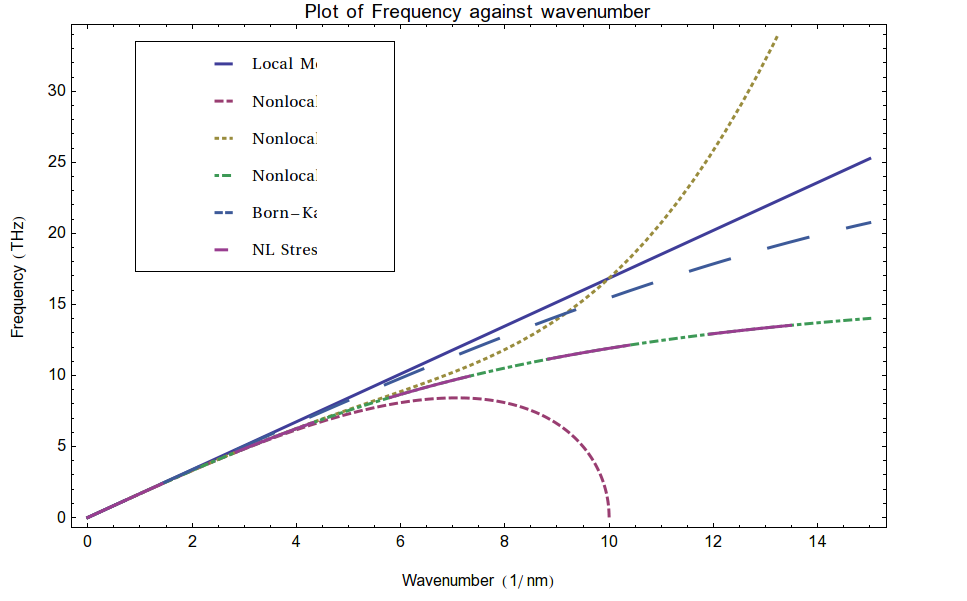
\includegraphics[scale=0.5]{final.png}
\end {figure}
\end {center}
